% sizes tiny scriptsize footnotesize small normalsize large Large LARGE huge Huge

\documentclass[presentation]{beamer}

\usetheme{JuanLesPins}
\usecolortheme{orchid}
\setbeamertemplate{headline}{}
\setbeamertemplate{navigation symbols}{}

\usepackage{subfig}
\usepackage{graphicx}
\usepackage[english]{babel}
\usepackage[latin1]{inputenc}
\usepackage{color}
\usepackage{listings}
\definecolor{mygreen}{rgb}{0,0.6,0}
\definecolor{mygray}{rgb}{0.5,0.5,0.5}
\definecolor{mymauve}{rgb}{0.58,0,0.82}

\lstset{
  backgroundcolor=\color{white},   % choose the background color; you must add \usepackage{color} or \usepackage{xcolor}; should come as last argument
  basicstyle=\footnotesize\ttfamily, % the size of the fonts that are used for the code
  breakatwhitespace=false,         % sets if automatic breaks should only happen at whitespace
  breaklines=true,                 % sets automatic line breaking
  captionpos=b,                    % sets the caption-position to bottom
  commentstyle=\color{mygreen},    % comment style
  deletekeywords={...},            % if you want to delete keywords from the given language
  escapeinside={\%*}{*)},          % if you want to add LaTeX within your code
  extendedchars=true,              % lets you use non-ASCII characters; for 8-bits encodings only, does not work with UTF-8
  frame=single,	                   % adds a frame around the code
  keepspaces=true,                 % keeps spaces in text, useful for keeping indentation of code (possibly needs columns=flexible)
  keywordstyle=\color{blue},       % keyword style
  morekeywords={*,...},            % if you want to add more keywords to the set
  numbers=none,                    % where to put the line-numbers; possible values are (none, left, right)
  numbersep=5pt,                   % how far the line-numbers are from the code
  numberstyle=\tiny\color{mygray}, % the style that is used for the line-numbers
  rulecolor=\color{black},         % if not set, the frame-color may be changed on line-breaks within not-black text (e.g. comments (green here))
  showspaces=false,                % show spaces everywhere adding particular underscores; it overrides 'showstringspaces'
  showstringspaces=false,          % underline spaces within strings only
  showtabs=false,                  % show tabs within strings adding particular underscores
  stepnumber=2,                    % the step between two line-numbers. If it's 1, each line will be numbered
  stringstyle=\color{mymauve},     % string literal style
  tabsize=2,	                   % sets default tabsize to 2 spaces
  title=\lstname,                  % show the filename of files included with \lstinputlisting; also try caption instead of title
  linewidth=10.7cm,
}

\usepackage{tikz}


% Add any additional packages you use in your presentation
% -----pack
% \usepackage{xxx}
% -----
\usepackage{ragged2e}
\usepackage{tikz}
\usetikzlibrary{shadows}

% Add your custom definitions etc., if required
% -----misc
% \newcommand{\xxx}[1]{[#1]}
% -----




\title{Reference counting}

\author[Miroslaw Blazej \&Miroslaw Blazej]
{%
   \texorpdfstring{
        \begin{columns}
            \column{.45\linewidth}
            \centering
            Miroslaw Blazej\\
            \href{mailto:blazej@student.agh.edu.pl}{blazej@student.agh.edu.pl}
            \column{.45\linewidth}
            \centering
            Michal Dygas\\
            \href{mailto:dygas@student.agh.edu.pl}{dygas@student.agh.edu.pl}
        \end{columns}
   }
   {Miroslaw \& Michal}
}
\institute[]{AGH University of Science and Technology}
\date{17-06-2020}


\begin{document}

\begin{frame}
  \titlepage
\end{frame}

\begin{frame}
  \frametitle{Introduction} 
  \justifying
 \textbf{Reference counting} is an \textbf{intuitive garbage collection} algorithm that \textbf{records in
each chunk the number of pointers that point to it}; when the number drops to
zero the chunk can be declared garbage; in a literal sense, reference counting collects garbage, unlike the other garbage collection algorithms, which actually collect
reachable chunks. In line with the name reference counting, we will call pointers
references in this section.
\end{frame}

\begin{frame}
  \frametitle{Rules}
  \justifying
    \begin{enumerate}
    \justifying
        \item When a chunk
is allocated from the heap, its reference count is initialized to one. 
        \item Whenever a
reference to the chunk is duplicated, its reference count is increased by one (incremented).
		\item Whenever a reference to the chunk is deleted, its reference
count is decreased by one (decremented).
		\item If the reference count drops to 0, the
chunk can be freed because it is no longer reachable
    \end{enumerate}  
\end{frame}


\begin{frame}
  \frametitle{Rules}
  \justifying
    \begin{block}{Implementation challenges}
        \begin{enumerate}
            \item keeping track of all
reference manipulations
            \item  recursively freeing chunks with zero reference count
        \end{enumerate}
  	\end{block}
\end{frame}

\begin{frame}
  \frametitle{keeping track of all
reference manipulations}
  \justifying
  The compiler inserts special code for all reference manipulations: incrementing
the reference count when a reference to a chunk is duplicated and decrementing it
when such a reference is deleted. 

	Besides assignment statements,
the compiler also has to add reference increasing code to parameter transfers, since
a reference that is passed as a parameter is effectively assigned to a local variable of
the called routine. Note that not all references in the running program are references to chunks on
the heap; many of them point to blocks in the program data area, and all referencecounting code must make sure it does not follow such references.
\end{frame}


\begin{frame}
  \frametitle{keeping track pseudocode}
  \justifying
  \begin{block}{title}
  \textbf{if} Points into the heap (q):\\ \hspace*{20pt} Increment q.referenceCount;\\ \textbf{if} Points into the heap (p):\\ \hspace*{20pt} Decrement p.referenceCount;\\ \hspace*{20pt} \textbf{if} p.referenceCount = 0:\\ \hspace*{40pt} FreeRecursively (p);
  \end{block}
\end{frame}  

\begin{frame}
  \frametitle{recursively freeing chunks pseudocode}
  \justifying  
  \begin{block}{title1}
  \textbf{procedure} FreeRecursively(Pointer); \\
\hspace*{20pt} \textbf{if} not IsPointerIntoHeap (Pointer): \textbf{return};\\
\hspace*{20pt} \textbf{if} Pointer.referenceCount != 0: \textbf{return};\\
\hspace*{20pt} \textbf{for each} i \textbf{in} 1 .. Pointer.numberOfPointers: \\
\hspace*{40pt} \textbf{if} IsPointerIntoHeap (Pointer.pointer [i]): \\
\hspace*{60pt} Decrement Pointer.pointer [i].referenceCount; \\
\hspace*{60pt} FreeRecursively(Pointer.pointer [i]); \\
\hspace*{20pt} FreeChunk(Pointer); \\
  \end{block}
\end{frame}

\begin{frame}
  \frametitle{Recursively freeing cons} 
  \justifying
      \begin{alertblock}{Cons}
        Recursion is, however, an unwelcome feature in a garbage collector since it requires an \textbf{unpredictable amount of stack space}. Having a garbage collector fail for lack of memory is kind of embarrassing, though, and several techniques
have been invented to avoid the problem. The best solution is using \textbf{pointer reversal}.
    \end{alertblock}
\end{frame}

\begin{frame}
  \frametitle{Identification techniques} 
  \justifying
  figures that will illustrate this algorithm
\end{frame}

\begin{frame}
  \frametitle{Identification techniques} 
  \justifying
  figures that will illustrate this algorithm
\end{frame}

\begin{frame}
  \frametitle{Algorithm issues} 
  \justifying
  \begin{alertblock}{Cons}
  	\begin{enumerate}
		\item efficiency
		\item memory fragmentation
		\item failes to reclaim a cyclic data structure 	
  	\end{enumerate}
  \end{alertblock}
\end{frame}


\begin{frame}
  \frametitle{Efficiency} 
  \justifying
The compiled code has
to monitor all reference manipulations, and each and every reference manipulation
requires the adjustment of the associated reference counts. This is a considerable
overhead in comparison to other garbage collection techniques that do not monitor
any pointer action and reclaim garbage chunks only when needed.
\end{frame}

\begin{frame}
  \frametitle{Memory fragmentation} 
  \justifying
The free list is augmented with the reclaimed chunks, but it remains fragmented. In principle
doing a compaction phase during a reference counting allocation request is possible,
but few reference counting garbage collectors go to such lengths.

    \begin{figure}
        \centering
            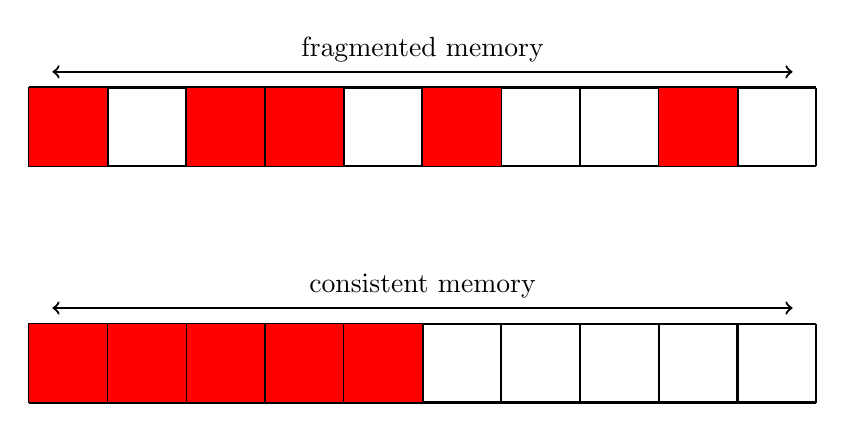
\begin{tikzpicture}
                \draw[thick, <->] (0.3, 1.2) -- (9.7, 1.2) node [midway, above, fill=white]{fragmented memory};
                
                \draw[thick] (0,0) grid (10,1);
                \filldraw[fill=red, draw=black] (0,0) rectangle (1,1);
                \filldraw[fill=red, draw=black] (2,0) rectangle (3,1);
                \filldraw[fill=red, draw=black] (3,0) rectangle (4,1);
                \filldraw[fill=red, draw=black] (5,0) rectangle (6,1);
                \filldraw[fill=red, draw=black] (8,0) rectangle (9,1);
                   
				\draw[thick, <->] (0.3, -1.8) -- (9.7, -1.8) node [midway, above, fill=white] {consistent memory};
				                   
                \draw[thick] (0,-2) grid (10,-3);
                \filldraw[fill=red, draw=black] (0,-2) rectangle (1,-3);
                \filldraw[fill=red, draw=black] (1,-2) rectangle (2,-3);
                \filldraw[fill=red, draw=black] (2,-2) rectangle (3,-3);
                \filldraw[fill=red, draw=black] (3,-2) rectangle (4,-3);
                \filldraw[fill=red, draw=black] (4,-2) rectangle (5,-3);
                
                
            \end{tikzpicture}
        \caption{Compaction example}
        \label{fig:compaction_example}
    \end{figure}

\end{frame}


\begin{frame}
  \frametitle{Cycles} 
  \justifying
The problem with reference counting is that it takes its decisions by considering
only one node in the graph at a time, and in order to reclaim a cyclic data structure all
nodes in the data structure should be considered as garbage together. Once reference
counting has failed to reclaim a cyclic data structure, the chunks involved will never
be reclaimed. This has the unfortunate effect that free space leaks away, which might
even cause the program to run out of free space when other garbage collectors would
be able to reclaim the cyclic structures and allow the program to continue.
\end{frame}


\begin{frame}
  \frametitle{Identification techniques} 
  \justifying
  \begin{figure}
      \centering
        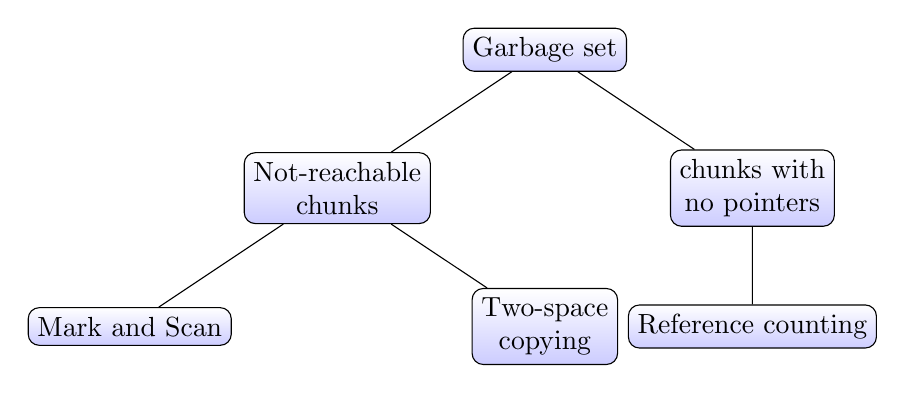
\begin{tikzpicture}[sibling distance=15em, level distance=5em, every node/.style = {shape=rectangle, rounded corners, draw, align=center, top color=white, bottom color=blue!20}]]
            \node {Garbage set}
                child {node {Not-reachable\\chunks}
                    child {node {Mark and Scan}}
                    child {node {Two-space\\copying}}
                }
                child {node {chunks with\\no pointers}
                    child {node {Reference counting}}
                };
        \end{tikzpicture}
      \caption{Garbage set identification techniques}
      \label{fig:my_label}
  \end{figure}
\end{frame}



\begin{frame}
  \frametitle{Identification techniques} 
  \justifying
  \begin{figure}
      \centering
        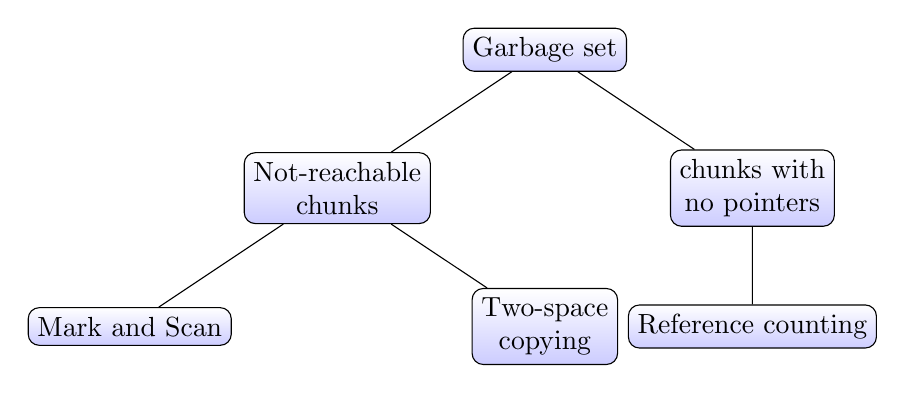
\begin{tikzpicture}[sibling distance=15em, level distance=5em, every node/.style = {shape=rectangle, rounded corners, draw, align=center, top color=white, bottom color=blue!20}]]
            \node {Garbage set}
                child {node {Not-reachable\\chunks}
                    child {node {Mark and Scan}}
                    child {node {Two-space\\copying}}
                }
                child {node {chunks with\\no pointers}
                    child {node {Reference counting}}
                };
        \end{tikzpicture}
      \caption{Garbage set identification techniques}
      \label{fig:my_label}
  \end{figure}
\end{frame}

\begin{frame}
    \frametitle{Reference counting: brief introduction}
    \justifying
    It is a really simple technique which, as the name suggests, keeps count of the number of references to each object.
    
    \begin{exampleblock}{Pros}
        \begin{itemize}
            \item Directly identifies garbage chunks
            \item Simple and reasonably efficient
        \end{itemize}
    \end{exampleblock}
    
    \begin{alertblock}{Cons}
        \begin{itemize}
            \item Requires all pointer actions to be monitored during program execution
            \item May not recover all garbage chunks
        \end{itemize}
    \end{alertblock}
\end{frame}

\begin{frame}
    \frametitle{Mark and scan: brief introduction}
    \justifying
    Mark and scan identifies reachable chunks and concludes that the rest is garbage.
    
    \begin{exampleblock}{Pros}
        \begin{itemize}
            \item Reasonably efficient and does not require pointer monitoring
        \end{itemize}
    \end{exampleblock}
    
    \begin{alertblock}{Cons}
        \begin{itemize}
            \item Quite complicated
            \item Recover all available memory
        \end{itemize}
    \end{alertblock}
\end{frame}

\begin{frame}
    \frametitle{Two-space copying: brief introduction}
    \justifying
    Two-space copying copies the reachable chunks from a memory region called "from-space" to a memory region called "to-space" -  the remaining space in to-space is a single free chunk. 
    
    \begin{exampleblock}{Pros}
        \begin{itemize}
            \item Very efficient
            \item Does not require pointer monitoring
            \item Moderately complicated
        \end{itemize}
    \end{exampleblock}
    
    \begin{alertblock}{Cons}
        \begin{itemize}
            \item Wastes half of the memory
        \end{itemize}
    \end{alertblock}
\end{frame}

\begin{frame}
    \frametitle{Short notice of compaction}
    \justifying
    Unfortunately locating and freeing proper chunks may not always be the final step as some of the techniques lead to \textbf{memory fragmentation}.This behaviour would cause significant problems in runtime as, even though, total free memory is satisfied the program cannot allocate data larger than the largest free chunk. Solution for this situation is called \textbf{compaction}. Compaction groups free memory blocks on one side and used on the other creating a single large free chunk. It is more complex and time consuming than just freeing the unused memory but it's fundamental as it makes the memory really \textit{available}.
\end{frame}

\begin{frame}
    \frametitle{Conceptual example of compaction}
    \begin{figure}
        \centering
            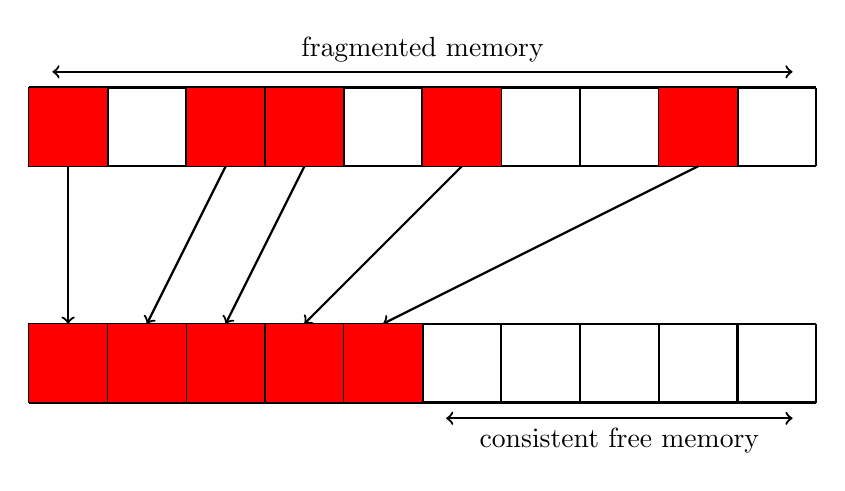
\begin{tikzpicture}
                \draw[thick, <->] (0.3, 1.2) -- (9.7, 1.2) node [midway, above, fill=white]{fragmented memory};
                
                \draw[thick] (0,0) grid (10,1);
                \filldraw[fill=red, draw=black] (0,0) rectangle (1,1);
                \filldraw[fill=red, draw=black] (2,0) rectangle (3,1);
                \filldraw[fill=red, draw=black] (3,0) rectangle (4,1);
                \filldraw[fill=red, draw=black] (5,0) rectangle (6,1);
                \filldraw[fill=red, draw=black] (8,0) rectangle (9,1);
                
                \draw[thick, ->] (.5, 0) -- (.5, -2);
                \draw[thick, ->] (2.5, 0) -- (1.5, -2);
                \draw[thick, ->] (3.5, 0) -- (2.5, -2);
                \draw[thick, ->] (5.5, 0) -- (3.5, -2);
                \draw[thick, ->] (8.5, 0) -- (4.5, -2);
                
                \draw[thick] (0,-2) grid (10,-3);
                \filldraw[fill=red, draw=black] (0,-2) rectangle (1,-3);
                \filldraw[fill=red, draw=black] (1,-2) rectangle (2,-3);
                \filldraw[fill=red, draw=black] (2,-2) rectangle (3,-3);
                \filldraw[fill=red, draw=black] (3,-2) rectangle (4,-3);
                \filldraw[fill=red, draw=black] (4,-2) rectangle (5,-3);
                
                \draw[thick, <->] (5.3, -3.2) -- (9.7, -3.2) node [midway, below, fill=white] {consistent free memory};
            \end{tikzpicture}
        \caption{Compaction example}
        \label{fig:compaction_example}
    \end{figure}
\end{frame}

\begin{frame}
    \frametitle{Fundamental types of garbage collection algorithms}
    \begin{figure}
        \centering
            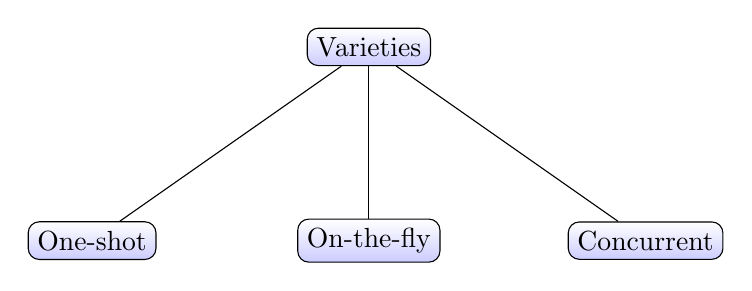
\begin{tikzpicture}[sibling distance=10em, level distance=7em, every node/.style = {shape=rectangle, rounded corners, draw, align=center, top color=white, bottom color=blue!20}]]
                \node {Varieties}
                    child {node {One-shot}}
                    child {node {On-the-fly}}
                    child {node {Concurrent}};
            \end{tikzpicture}
        \caption{Garbage collection algorithm types}
        \label{fig:gc_algo_types}
    \end{figure}
\end{frame}

\begin{frame}
    \frametitle{One-shot}
    \justifying
    This group of algorithms is fairly simple since the garbage collector is in full control while running, however, because of that its execution can be disruptive. That's why it's more suitable for compilers than interactive programs.
    
    \begin{block}{Depicted routine}
        \begin{enumerate}
            \item Starting the garbage collector
            \item Execution till completion while in full control of all chunks
            \item Returning
        \end{enumerate}
    \end{block}
\end{frame}

\begin{frame}
    \frametitle{On-the-fly}
    \justifying
    Some garbage collector actions are performed at each call of Malloc and/or Free. These actions make some local modifications to the chunk structure to increase the probability of finding a free chunky when needed.
    
    \begin{itemize}
        \item On-the-fly garbage collectors are usually much more difficult to construct than one-shot garbage collectors, but are smoother and less disruptive in their operation.
        \item They may still need a one-shot garbage collector as back-up for situations in which they cannot cope with the demand.
    \end{itemize}
\end{frame}


\begin{frame}
    \frametitle{Concurrent}
    \justifying
    In concurrent approach garbage collector \textbf{runs on a second processor}, different from the one that runs the program. It runs continuously and concurrently, and tries to keep memory garbage-free. Unfortunately, concurrent garbage collection is sometimes also called on-the-fly, in spite of the fact that this term suggests one agent rather than two.
\end{frame}


\begin{frame}
    \frametitle{Implementation of garbage set techniques}
    \begin{figure}
        \centering
            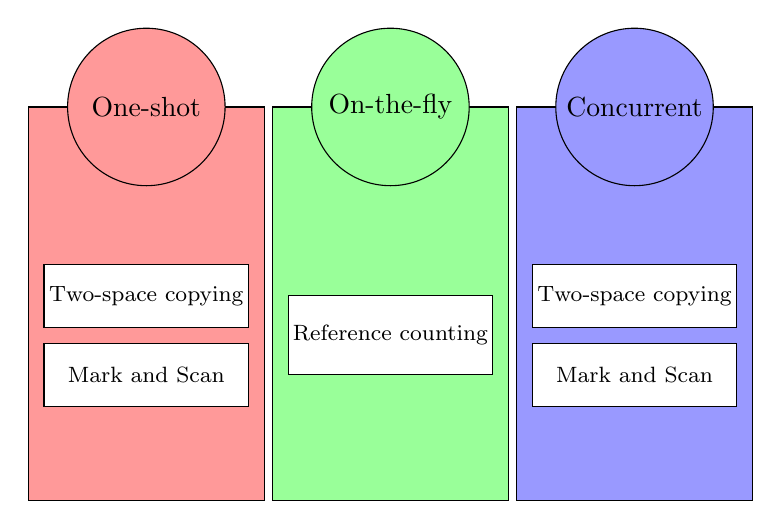
\begin{tikzpicture}
                \filldraw[fill=red!40!white, draw=black] (0,0) rectangle (3,5);
                \filldraw[fill=green!40!white, draw=black] (3.1,0) rectangle (6.1,5);
                \filldraw[fill=blue!40!white, draw=black] (6.2,0) rectangle (9.2,5);
                
                \filldraw[fill=red!40!white, draw=black] (1.5,5) circle [radius=1] node {One-shot};
                \filldraw[fill=green!40!white, draw=black] (4.6,5) circle [radius=1] node {On-the-fly};
                \filldraw[fill=blue!40!white, draw=black] (7.7,5) circle [radius=1] node {Concurrent};
                
                \filldraw[fill=white, draw=black] (0.2,1.2) rectangle (2.8,2) node[pos=.5, font=\footnotesize] {Mark and Scan};
                \filldraw[fill=white, draw=black] (6.4,1.2) rectangle (9,2) node[pos=.5, font=\footnotesize] {Mark and Scan};
                
                \filldraw[fill=white, draw=black] (0.2,2.2) rectangle (2.8,3) node[pos=.5, font=\footnotesize] {Two-space copying};
                \filldraw[fill=white, draw=black] (6.4,2.2) rectangle (9,3) node[pos=.5, font=\footnotesize] {Two-space copying};
                
                \filldraw[fill=white, draw=black] (3.3,1.6) rectangle (5.9,2.6) node[pos=.5, font=\footnotesize] {Reference counting};
            \end{tikzpicture}
        \caption{Categorization of different garbage set implementations}
        \label{fig:gc_techniques}
    \end{figure}
\end{frame}


\begin{frame}
    \frametitle{Getting to know pointers before implementation}
    \begin{block}{We can distinguish two kinds of pointers:}
        \begin{itemize}
            \item Direct - A chunk of the memory is reachable for the program using just this one (direct) pointer.
            \item Indirect - A chunk of the memory is reachable for the program using some other (indirect) pointer.
        \end{itemize}
    \end{block}
    
    \justifying
    The directly available pointers can be located in various places, depending on the implementation. These places may include the global/local variables, registers and perhaps many others.
\end{frame}

\begin{frame}
    \frametitle{Non-heap memory and root set}
    \begin{block}{Non-heap memory}
    \justifying
    Also called the program data area, and consists of the memory that is directly accessible to the program code.
    \end{block}
    
    \begin{block}{Root set}
    \justifying
    Is a conceptual notion that depicts the set of pointers in the program data area. Usually it's not implemented but only conceptually present in the garbage collector's program code. It's worth noting that it isn't a list of pointer values but just the set of all pointers in the program data area.
    \end{block}
\end{frame}

\begin{frame}
    \frametitle{Garbage collection problem decomposition}
    \justifying
    The pointers from the root set may point to chunks in the heap (controlled by the garbage collector) what makes this chunks reachable. Those reachable chunks can obviously contain pointers to other areas in the heap which are then reachable as well.
    \\~\\
    That's why we can divide the problem of finding all reachable chucks (thus problem of the garbage collection) into three subproblems:
    
    \begin{enumerate}
        \item Finding all pointers in the program data area with their types (so finding the root set)
        \item Finding all pointers in a given chunk with their types
        \item Finding all reachable chunks using the information from subproblems 1 and 2
    \end{enumerate}
\end{frame}

\begin{frame}
    \frametitle{Garbage collection problem decomposition}
    \justifying
    To solve subproblems 1 and 2 the garbage collector needs compiler support. It has to deliver information about the pointer layout of the program data area and each chunk type. We cover this 
    scenarios in the next slides.
    \\~\\
    Garbage collection algorithms themselves can be treated as the solutions for the third subproblem which is usually solved by implementing them as runtime routines.
\end{frame}

\begin{frame}
    \frametitle{Root set and heap example}
    \begin{figure}
        \centering
            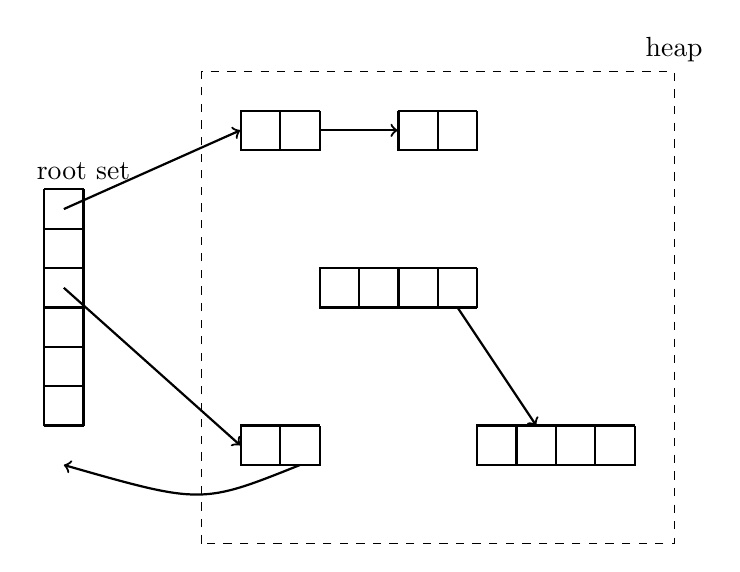
\begin{tikzpicture}
                \draw[thick, step=0.5cm] (0,1.49) grid (.5,4.5) node [fill=white, above]{root set};
                \draw[dashed] (2,0) rectangle (8,6) node[fill=white, above]{heap};
                
                \draw[thick, step=0.5cm] (2.49,4.99) grid (3.5,5.5);
                \draw[thick, step=0.5cm] (4.49,4.99) grid (5.5,5.5);
                \draw[thick, step=0.5cm] (3.49,2.99) grid (5.5,3.5);
                \draw[thick, step=0.5cm] (2.49,0.99) grid (3.5,1.5);
                \draw[thick, step=0.5cm] (5.49,0.99) grid (7.5,1.5);
                
                \draw[thick, ->] (.25, 4.25) -- (2.49, 5.25);
                \draw[thick, ->] (3.5, 5.25) -- (4.49, 5.25);
                \draw[thick, ->] (.25, 3.25) -- (2.49, 1.25);
                %\draw[thick, ->] (3, 1.25) -- (0.25, 1);
                \draw[thick, ->] (3.25, 1) ..controls (2, .5) .. (0.25, 1);
                \draw[thick, ->] (5.25, 3) -- (6.25, 1.5);
            \end{tikzpicture}
        \caption{A root set and a heap with reachable and unreachable chunks}
        \label{fig:my_label}
    \end{figure}
\end{frame}

\begin{frame}
    \frametitle{Pointer consistency}
    \justifying
    To do its job the garbage collector has to be able to understand all the pointers that it deals with, since it will follow any pointer to find the garbage. 
    \\~\\
    That's why the pointer  consistency (also called pointer validity) must be ensured (usually by the language definition and the compiler).
\end{frame}

\begin{frame}
    \frametitle{Compilers support for garbage collection}
    \justifying
    To give a proper support for the garbage collection process compiler has to:
    
    \begin{enumerate}
    \justifying
        \item \textbf{Provide the root set} and information about the \textbf{pointer layout} of each chunk to the garbage collector  (the pointer layout of a chunk C describes the position of each pointer P in the chunk, together with the type of the chunk that P points to). 
        \item Make sure that all \textbf{reachable pointers}, both in the program data area and in the heap, \textbf{are valid} when the garbage collector is activated.
    \end{enumerate}
\end{frame}

\begin{frame}
    \frametitle{Chunks pointer layout}
    \justifying
    The compiler is in full control of the layout of chunks. The only problem is how to transfer the knowledge of the pointer layout to the garbage collector - chunks needs to be \textbf{self-descriptive}.
    
    \begin{block}{Two common approaches:}
        \begin{itemize}
            \item Chunks can carry their pointer layout information in each copy
            \item They can all have the same layout
        \end{itemize}
    \end{block}
\end{frame}

\begin{frame}
    \frametitle{Storing chunks pointer layout}
    \justifying
    To properly store the pointer layout compiler can:
    
    \begin{enumerate}
        \item Generate a \textbf{bitmap} for each chunk type. With this method, chunks must be self-descriptive, since just having the pointer must be sufficient for the garbage collector to continue. So each chunk must either contain its bitmap or a pointer to its bit map
        \item Generate a specific \textbf{routine} for each chunk type, which calls a garbage collector routine passed as a parameter for each pointer inside the chunk.
        \item The compiler can organize the chunks to start off with an \textbf{array containing all pointers}, followed by the other data types. With this organization, the collector only has to know the location of the pointer array and the total number of pointers inside the chunk.
    \end{enumerate}
\end{frame}

\begin{frame}
    \frametitle{Program data pointer layout}
    \justifying
    The root set is supplied by running a \textbf{library routine} that \textbf{scans the program data area} and calls a specific garbage collection routine for each pointer the program data area contains. It is then up to the specific garbage collection routine to see if the pointer is interesting and perform the proper actions. To perform its task, the library routine must be able to find all pointers in the program data area, with their types, and be sure each pointer is valid.
    \\~\\
    The problem is that the pointer layout of the program data area, unlike that of chunks, is complicated and dynamically variable.
\end{frame}

\begin{frame}
    \frametitle{Program data area}
    \justifying
    The program data area consists of the \textbf{global data area} and a stack holding one or more \textbf{stack frames} or \textbf{activation records}. The pointer layout of the global data area is known and constant, although it may be distributed over several source program modules. To know the pointer layout of the stack, the garbage collector has to know which activation records it contains, and what the pointer layout of each activation record is. 
    \\~\\
    Both pieces of information are dynamic, so activation records must be also \textbf{self-describing}.
\end{frame}

\begin{frame}
    \frametitle{Conclusion}
    \justifying
    As you can see garbage collection can be a really complex field. It consists of seemingly simple ideas which require a lot of work and knowledge to be properly implemented.
    \\~\\
    We hope that this presentation borough this matter closer to you and made you familiar with basic concepts of the garbage collection and basic garbage collection algorithms.
\end{frame}

\begin{frame}
    \frametitle{Bibliography}
    \justifying
    Our research was based on the book:\\Dick Grune et al. "\textit{Modern Compiler Design}"
\end{frame}

\end{document}
